\section{Theorie}
\label{sec:Theorie}
\subsection{Grundlagen}
\label{sec:grundlagen}
Beugung tritt immer dann auf, wenn Licht auf ein Hindernis bzw. ein Öffnung trifft, welche von den Abmessungen die Größenordnung der Wellenlänge $\lambda$ des Lichts
besitzt. Die Beugung kann dabei nicht mehr wie Reflexion oder Berechnung über die Strahlenoptik beschrieben werden, sondern wird als Wellenvorgang
beschrieben.
\\\noindent
Elementar für die Beschreibung des Lichts ist dabei das Huygenssche Prinzip. Dieses besagt, dass jeder Punkt der Wellenfront wieder als Elementarwelle
aufgefasst werden kann. Durch die Superposition dieser Elementarwellen ergibt sich dann die neue Wellenfront. Aus diesem Prinzip werden in den nachfolgenden
Kapiteln die Beugungsbilder der Fernfeldbeugung (Frauenhoferbeugung) und der Nahfeldbeugung (Fresnelbeugung) hergeleitet.

\subsection{Beugung am Einzelspalt}
\label{sec:einzel}
Trifft eine Wellenfront auf ein Hindernis mit einem Spalt, so kann nach dem Huygensschen Prinzip jeder Punkt der Spaltöffnung als Quelle für eine Elementarwelle
verstanden werden. Diese Wellen breiten sich dann kugelförmig aus und interferieren miteinander. Wichtig für die Interferenz und damit das Beugungsbild ist,
dass das Licht kohärent ist, also dass zwischen zwei Wellenzügen eine feste Phasenbeziehung besteht. Ansonsten bildet sich kein stabiles Interferenzmuster.
\\\noindent
Es wird bei der Beugung zwischen zwei Näherungen unterschieden,
die nun weiter erläutert werden.

\subsubsection*{Fraunhoferbeugung}
Die Fraunhoferbeugung nähert die Entfernung der Lichtquelle von dem Spalt als unendlich, weswegen die Lichtstrahlen alle parallel nebeneinander verlaufen, also
eine ebene Wellenfront bilden. Somit werden alle Strahlen unter dem selben Winkel $\phi$ gebeugt. In Abbildung \ref{fig:frauenhofer} ist der Verlauf der
Lichtstrahlen skizziert.
\begin{figure}[H]
    \centering
    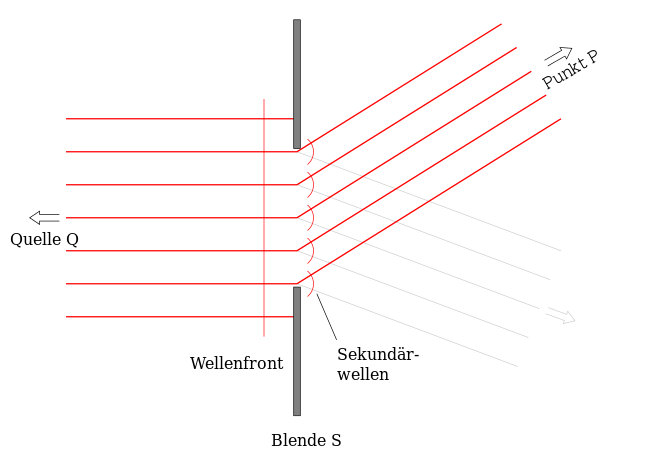
\includegraphics[scale = 0.45]{pictures/frauenhofer.png}
    \caption{Fraunhoferbeugung am Einzelspalt. \cite{AP02}}
    \label{fig:frauenhofer}
\end{figure}
\noindent

\subsubsection*{Fresnelbeugung}
Bei der Fresnelbeugung ist der Abstand der Lichtquelle zu dem Spalt endlich. Die Wellenfront ist also nicht eben, sondern kugelförmig. Die Lichtstrahlen sind
demnach nicht parallel und werden unter unterschiedlichen Winkeln gebeugt. Dadurch ist die Fresnelbeugung mathematisch deutlich anspruchsvoller als die
Frauenhoferbeugung. In Abbildung \ref{fig:fresnel} ist die Fresnelbeugung noch einmal schematisch dargestellt.
\begin{figure}[H]
    \centering
    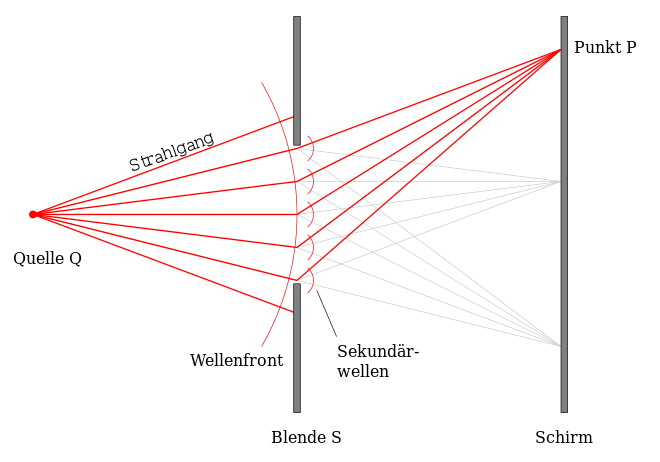
\includegraphics[scale = 0.45]{pictures/fresnel.png}
    \caption{Fresnelbeugung am Einzelspalt. \cite{AP02}}
    \label{fig:fresnel}
\end{figure}
\noindent

\subsubsection*{Berechnung der Intensitätsverteilung}
\label{sec:intensität}
Da die Fraunhoferbeugung aufgrund der gleichen Beugungswinkel mathematisch einfacher ist, wird im Folgenden die Intensitätsverteilung $I(\phi)$
nur für die Fernfeldnäherung hergeleitet. Zudem wird ein Spalt betrachtet, dessen Breite $b$ sehr viel kleiner als seine Länge ist. Somit findet
die Beugung in recht genauer Näherung nur in einer Dimension statt.
\\\noindent
Wie bereits beschrieben lassen sich die einfallenden Wellen als ebene Wellen nähern. Die Amplitude der Welle ist gegeben durch
\begin{equation*}
    A(z,t)=A_0\exp{(i(\omega t-2\pi z/\lambda))}    ,
    \label{eqn:ebenewelle}
\end{equation*}
wobei das Koordinatensystem entsprechend zu Abbildung \ref{fig:frauenhofer2} gelegt ist. Weiter in der Abbildung zu sehen ist, dass zwei
Lichtstrahlen im Abstand $x$ von einander, einen Wegunterschied $s$ besitzen. Dieser führt zu einem Phasenunterschied $\delta$, der durch
\begin{equation*}
    \delta=\frac{2\pi s}{\lambda}=\frac{2\pi x \sin{\phi}}{\lambda}
    \label{eqn:phase}
\end{equation*}
beschrieben werden kann.

\begin{figure}[H]
    \centering
    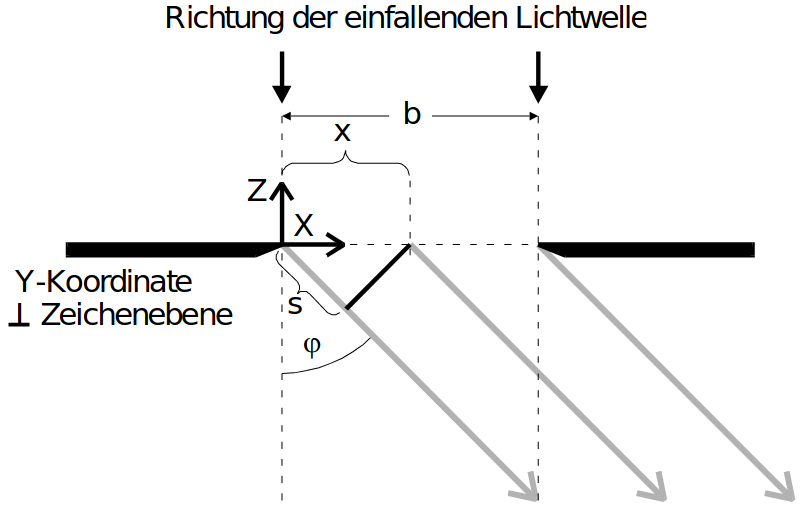
\includegraphics[scale = 0.45]{pictures/frauenhofer2.png}
    \caption{Skizze zum Gangunterschied zweier Lichtstrahlen bei derFrauenhoferbeugung. \cite{AP01}}
    \label{fig:frauenhofer2}
\end{figure}

\noindent
Nach dem Huygensschen Prinzip kann nun die Amplitudenfunktion $B(z,t,\phi)$ bestimmt werden, indem über alle Elementarwellen
in der Spaltenöffnung summiert wird. Wegen der infinitisimalen Breite der Strahlen und der kontinuierlichen Verteilung geht die Summe in ein
Integral über die Spaltöffnung über
\begin{equation*}
    B(z,t,\phi)=A_0\int_0^b{\exp{\left(i\left(\omega t-\frac{2\pi z}{\lambda}+\delta\right)\right)}\symup{dx}}    .
\end{equation*}
Dieses Integral lässt sich lösen zu
\begin{equation*}
    B(z,t,\phi) = A_0\exp{\left(i\left(\omega t-\frac{2 \pi z}{\lambda}\right)\right)}
                \cdot\exp{\left(\frac{\pi \symup{i} b \sin{(\pi)}}{\lambda}\right)}
                \cdot \sinc(\eta)
\end{equation*}
mit
\begin{equation*}
    \eta=\frac{\pi b \sin{\phi}}{\lambda}   .
\end{equation*}
$\sinc{\eta}$ ist dabei der Kardinalsinus. Die beiden Exponentialfunktionen sind aufgrund ihrer Komplexwertigkeit bei dem Experiment nicht von Belang,
da ohnehin nur die Intensität $I(\phi)\propto |B(z,t,\phi)|^2$ gemessen werden kann. Da der Betrag einer komplexen Exponentialfunktion $\num{1}$ ist, muss
demnach nurnoch
\begin{equation}
    B(\phi)=A_0b\sinc{\eta}
    \label{eqn:B}
\end{equation}
betrachtet werden. Die Nullstellen der Funktion \eqref{eqn:B} liegen bei $\pm n\lambda/b$ mit $n \in \mathbb{N}$.
\\\noindent
Wie bereits angedeutet gilt
\begin{equation}
    I(\phi)\propto B(\phi)^2=
    A_0b^2\sinc^2{\left(\frac{\pi b \sin{\phi}}{\lambda}\right)}
    \geq 0  .
    \label{eqn:intensität1}
\end{equation}
Somit liegen bei den Nullstellen der Amplitudenfunktion \ref{eqn:B} Minima in der Intensität $I(\phi)$ vor. Die Höhe der Maxima fällt in
Näherung mit $\phi^2$ ab.

\begin{figure}[H]
    \centering
    \includegraphics[scale = 1.0]{pictures/intensität1.png}
    \caption{Theoriekurve der Intensitätsverteilung, wobei $\alpha\equiv\phi$ und $d\equiv b$. \cite{AP03}} %Hier vielleicht doch lieber gleich??
    \label{fig:frauenhofer3}
\end{figure}

\subsection{Beugung am Doppelspalt}
\label{sec:doppel}
Für einen Doppelspalt kann die Intensität $I(\phi)$ recht analog bestimmt werden. Der Doppelspalt wird dabei als Überlagerung zweier Einzelspalte im
Abstand $s$ verstanden. In Abbildung \ref{fig:doppel} ist ein solcher Doppelspalt skizziert.
\begin{figure}[H]
    \centering
    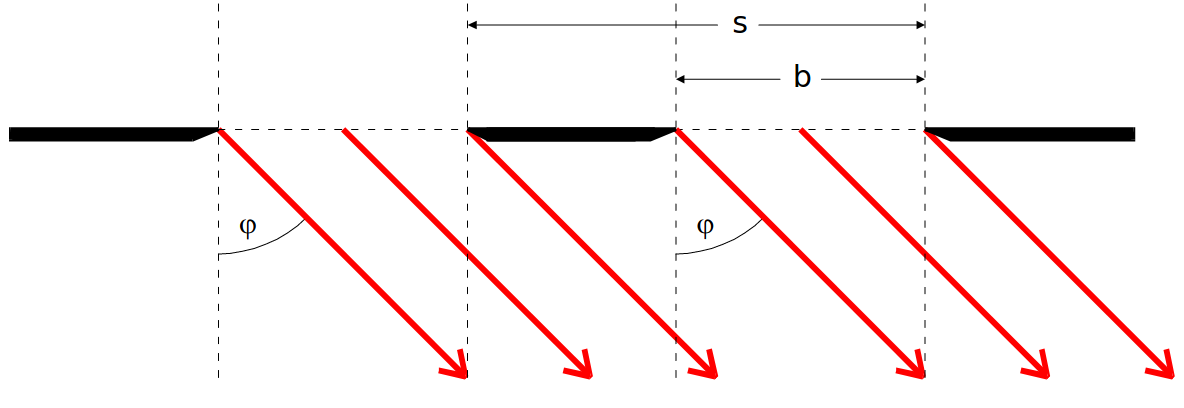
\includegraphics[scale = 0.4]{pictures/doppel.png}
    \caption{Schematische darstellung der Beugung am Doppelspalt. \cite{AP01}}
    \label{fig:doppel}
\end{figure}

\noindent
Die Intensitätsverteilung ist dann gegeben durch
\begin{equation}
    I_d(\phi)\propto B_d(\phi)^2
    =4\cdot \cos{\left(\frac{\pi s\sin{\phi}}{\lambda}\right)}\cdot \sinc^2{\left(\frac{\pi b \sin{\phi}}{\lambda}\right)}  .
    \label{eqn:intensität2}
\end{equation}
Im Vergleich zu der Intensitätsverteilung \eqref{eqn:intensität1} des Einzelspalts ist bei der des Doppelspalts \eqref{eqn:intensität2} ein
$\cos^2$-Term hinzugekommen. Dadurch entstehen zusätzliche Minima an den Stellen $\arcsin{((2k+1)/2s)}$ mit $k\in\mathbb{N_0}$. Die entstehende
Intensitätsverteilung des Doppelspalts \eqref{eqn:intensität2} ist in Abbildung \ref{fig:intensität2} dargestellt. Die Einhüllende ist die Intensitätsverteilung
\ref{eqn:intensität1} des Einzelspalts.
\begin{figure}[H]
    \centering
    \includegraphics[scale = 1.0]{pictures/intensität2.png}
    \caption{Intensitätsverteilung eines Doppelspalts mit willkürlicher Skala. Die Einhüllende ist die Verteilung eines Einzelspalts. \cite{AP04}}
    \label{fig:intensität2}
\end{figure}

\subsection{Berechnung des Intensitätsverteilung durch Fouriertransformation}
\label{sec:fourier}
Die Amplitudenverteilung kann auch durch eine Fouriertransformation berechnet werden. Dieser Weg ist in sofern eleganter, dass er sich ohne
größeren Aufwand auf mehrere Dimensionen erweitern lässt. Die Berechnung der Amplitudenfunktion wird nachfolgend kurz erläutert.
\\\noindent
Das Huygenssche Prinzip beruht auf der Superposition einzelner Elementarwellen. Diese Superposition kann wie in Abschnitt \ref{sec:einzel}
angedeutet durch das Integral
\begin{equation}
    g(\xi)=\int_{-\infty}^{\infty}f(x)\exp{(ix\xi)}\symup{dx}
    \label{eqn:fouriertrafo}
\end{equation}
erfolgen. Dabei ist die Funktion $f(x)$ die Aperturfunktion, also die Amplitudenverteilung der einfallenden Welle in der Beugungsebene.
Der Faktor $\exp{(ix\xi)}$ beschreibt dann gerade die Phasendifferenz einer Elementarwelle mit Quelle $x$ zu der ausgehenden Welle von $x=0$.
Das Integral \eqref{eqn:fouriertrafo} beschreibt nun gerade die Fouriertransformierte $g(\xi)=\hat{f}(\xi)$ der Aperturfunktion. Das Auswerten
des Integrals ergibt
\begin{equation*}
    g(\xi)=\frac{2A_0}{\xi}\exp{\left(\frac{i\xi b}{2}\right)}\sin{\left(\frac{\xi b}{2}\right)}    .
\end{equation*}
Mit der Definition
\begin{equation*}
    \xi=\frac{2 \pi \sin{\phi}}{\lambda}
\end{equation*}
wird der Zusammenhang zu Gleichung \eqref{eqn:B} deutlich.
